\appendix

\section{Calibration Solutions for the sky model tests }\label{ap:calib_solutions}
The output of the calibration step is a data set corrected for direction independent effects, as well as a set of calibration solutions. Figures \ref{fig:skymodel_rcalib_004_03} and \ref{fig:skymodel_rcalib_08_15} show the calibration solutions for core station obtained when calibrating with  sky models with minimum flux cutoffs of0.05, 0.3, 0.8 and 1.5Jy.

\begin{figure}
    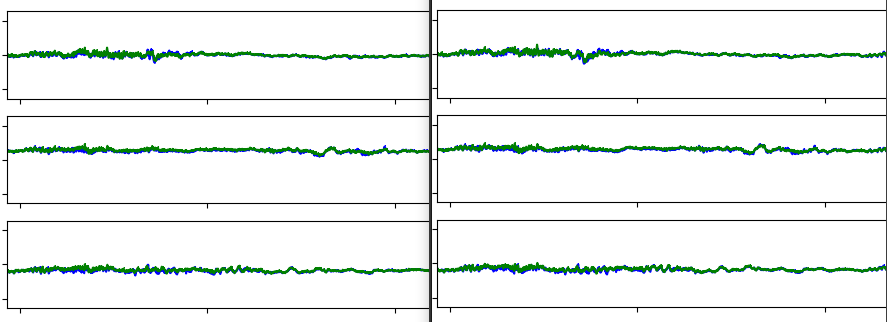
\includegraphics[width=0.95\linewidth]{figures/005_and_03_solutsions_CS003HBA0_CS003HBA1_CS004HBA0.png}
      \caption{The calibration (phase) solutions for the test dataset obtained when calibrating with sky models of 0.05 Jy cutoff (left) and 0.3Jy cutoff (right). The data shows the phase solutions for baselines including stations CS003HBA0, CS003HBA1 and CS004HBA0, with respect to the reference station, CS001HBA0.}
	\label{fig:skymodel_rcalib_004_03}
\end{figure}


\begin{figure}
    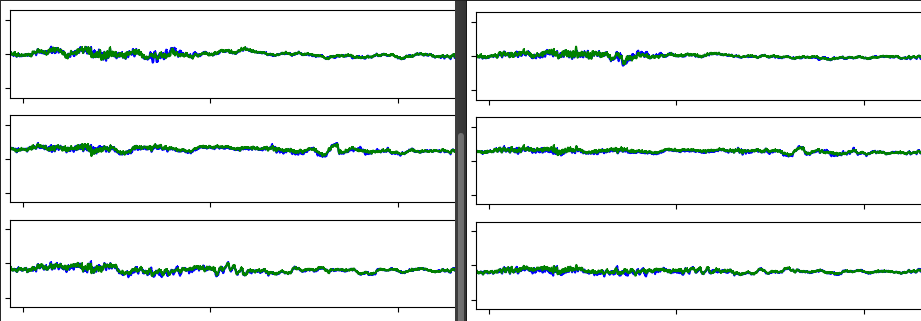
\includegraphics[width=0.95\linewidth]{figures/08_and_15_solutsions_CS003HBA0_CS003HBA1_CS004HBA0.png}
      \caption{The calibration (phase) solutions for the test dataset obtained when calibrating with sky models of 0.8 Jy cutoff (left) and 1.5Jy cutoff (right). The data shows the phase solutions for baselines including stations CS003HBA0, CS003HBA1 and CS004HBA0, with respect to the reference station, CS001HBA0.}
	\label{fig:skymodel_rcalib_08_15}
\end{figure}



%\subsection{Shell session isolation}

%\subsection{Setting up for future pipelines}


